\section{Improved the SFC system}
\label{sec:sfc}

\url{gitolite@nedm.psi.ch:babySFC}

\textit{Overview}: Surrounding Field Compensation \cite{Franke2013, Rawlik2018a} system, or the \textbf{SFC}, is an important part of the n2EDM experimental setup. Its purpose is to sustain a magnetic field of a desired magnitude and direction in the measurement area. This goal is achieved by controlling the currents in a set of the magnetic coils \cite{Rawlik2018} in order to respond to the changes in the magnetic fields of the environment. The aim of the Feature \ref{sec:sfc} is similar to the one introduced in the Feature \ref{sec:rm-proxy}. SFC needed to be converted into a regular DAQ node that can be controlled over the SCPI connection and that can feed the COM handler with the experimental data in a compliant \cite{Bison2018} way and shape.

\subsection{SCPI interface}
\label{subsec:sfc_scpi}

\textit{Motivation}: we would like to replace an existing GUI control capabilities with a set of the SCPI commands in order to predictably govern the state of execution and the setup parameters of the SFC system.

\begin{figure}[h]
	\centering
	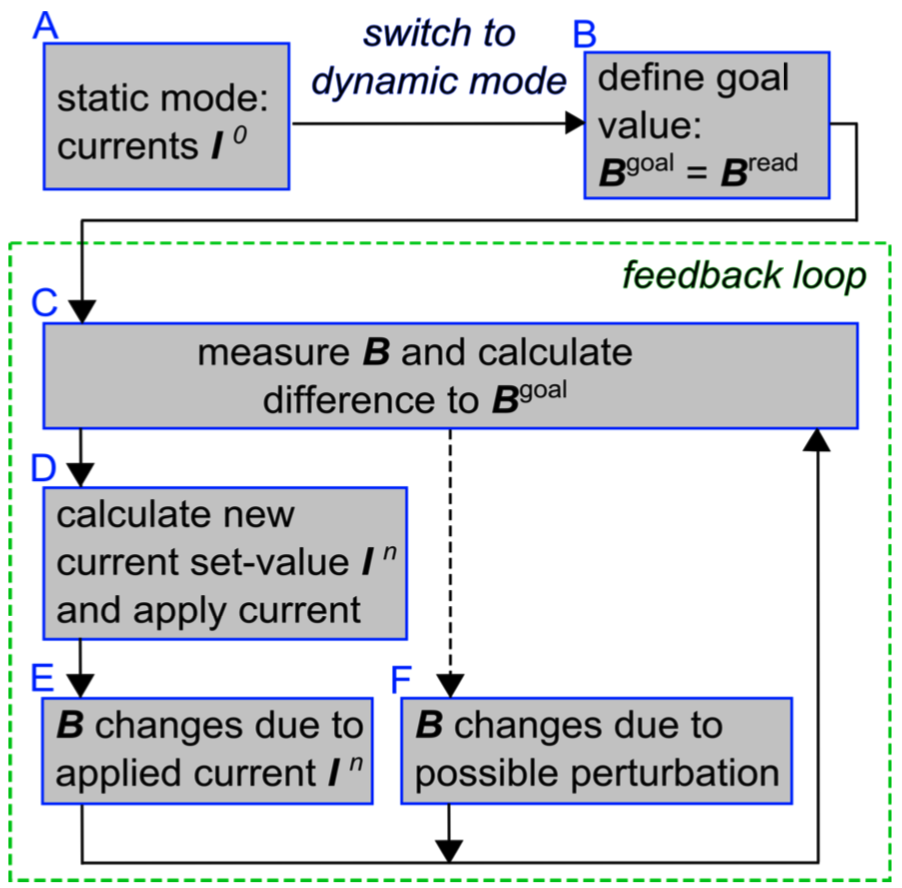
\includegraphics[width=\textwidth]{img/sfc_algorithm}
	\caption{Schematic structure of the SFC lifecycle taken from \cite{Franke2013}.}
	\label{fig:sfc_algorithm}
\end{figure}

\textit{Requirements}: as described in great details in \cite{Franke2013} the SFC system can run in either \texttt{STATIC} or \texttt{DYNAMIC} mode. While in \texttt{STATIC} the system is time-independent and fully characterised with $I^0$ which is a vector with every individual component defining a ratio of the immediate set current in the corresponding coil to the current at the nominal generated magnetic field. When switched to the \texttt{DYNAMIC} mode the new $I^n$ is recalculated on every iteration based on the difference between the expected and the measured fields. An overview of the SFC behaviour in the different modes can be found on the Figure \ref{fig:sfc_algorithm}.

We introduce the following 2 commands to control the experimental setup:
\begin{itemize}
	\item \texttt{MODE <STATIC|DYNAMIC>} that switches between the execution modes.
	\item{
		\texttt{COIL index, current} to modify the components of the $I^0$.
		\begin{itemize}
			\item \texttt{index}, required integer --- an index of the corresponding coil. The coil index itself is derived from the coil's position in the config file. Indices start with 1. Any index that is outside the $I^0$ boundaries is ignored and an error message is printed.
			\item \texttt{current}, required float --- a ratio of the current to be set to the maximal current. However at the moment there are no checks and one can set this value to be greater than 1 if desired.
		\end{itemize}
	}
\end{itemize}

\textit{Implementation details}: existing SFC software communicates with the main \texttt{babySFC.jl} module via a ZeroMQ connection. This endpoint was kept for the sake of the compatibility. However it is important to notice that these ZeroMQ messages simply contain the \textbf{name of the variable} and its new value to be set. Thus one needs to make sure that until the legacy scripts are properly modified to work with the SCPI commands it is necessary to keep the variable name that defines $I^0$ to be \texttt{logicalI}.

\subsection{Data interface}
\label{subsec:sfc_data}

\textit{Motivation}: in the n2EDM DAQ system the COM handler is responsible for writing the data to the disk for the further analysis thus it is the job of the SFC to bundle it into a binary message and send the package over TCP.

\textit{Requirements}:














